
\documentclass[11pt, oneside]{article}
\usepackage{geometry} 
\geometry{a4paper} 
%\usepackage[parfill]{parskip}  % Activate to begin paragraphs with an empty line rather than an indent
\usepackage{graphicx}	
\graphicspath{ {../figures/} }
\usepackage{amssymb}
\usepackage{xcolor}
\usepackage{listings}

\pagenumbering{gobble}

\definecolor{codegray}{gray}{0.88}
\newcommand \Rcode[1]{{\texttt{\colorbox{codegray}{#1}}}}
%\newcommand \Rcode[1]{{\texttt{{#1}}}}

\title{Finding Pulsars with Generalised Linear Models}
%\author{Robson Edwards}
\author{Matriculation Number 150017877}
\date{November 27, 2018}

\begin{document}

\maketitle

\section{Executive Summary}

We analyse a dataset which contains information on the emission spectra of a number of ``pulsar candidates''. Pulsars are a rare and interesting variety of neutron star which exhibit certain radio signals which allow them to be detectable from Earth. However, many similar signals come from radio interference and noise. Seeking to separate true pulsars from spurious candidates, we inspect the data and devise a number of Generalised Linear Models which allow us to predict pulsar presence based on signal characteristics. We select our best model and compare it to an alternative classification approach.  

\section{Introduction}

Pulsars are a rare and interesting type of neutron star which rotate at a fast rate and transmit a periodic signal which can be detected by large radio telescopes on Earth. However, similar signals can be generated by noise or radio-frequency interference. Hence, classification of genuine pulsars from so-called ``pulsar candidates'' is an area of considerable scientific interest.\cite{data}

Other, more recent (relative to GLMs) machine-learning approaches have been applied to this problem with comparable results. We will return to this point later. 

Note that throughout this paper, we are more worried about false negatives than false positives. The cost of a false negative is potentially missing out on a pulsar discovery, whereas the cost of a false positive is the time it takes a researcher or grad student to inspect the example and reject it by hand. This could potentially change if the number of candidates we wish to inspect increases drastically. 

\section{Methods}

What follows is a description of the data, followed by our methods for model formulation and selection as well as our motivations and justifications for the steps taken herein. 

\subsection{Data}
\label{subsec:data}

The data are the HTRU2 dataset, ``which describes a sample of pulsar candidates collected during the High Time Resolution Universe Survey.'' \cite{data} It was downloaded from the UC Irvine Machine Learning repository.

The data consist of 17,898 ``pulsar candidates'' (rows). For each candidate we have eight continuous variables (henceforth V1 through V8) and one binary class variable, for a total of nine columns. V1 through V4 describe features of the integrated profile of the emission pattern from different pulsar candidates. V5 through V8 describe features of the candidate's DM-SNR curves (dispersion measure and signal-to-noise ratio). \cite{data} While the specific details of these eight variables are interesting, they are outside the scope of this course and paper. The last variable is binary and labels of the candidate's class (authentic pulsar or spurious candidate). Fortuitously, every pulsar candidate is labelled. Of the candidates, 1,639 are genuine pulsars and 16,259 are spurious. We treat this as a supervised learning problem, where the eight explanatory variables are used to predict class. 

We plot relationships between the eight explanatory variables in Figure {\ref{fig:scatter}}. It can be seen, roughly speaking, that the pulsars (cyan) and non-pulsars (orange) are well-separated on many axes. Hence, we imagine that we could address our prediction problem with a binomial GLM. 

There are at least two problems with the data. First, the explanatory variables are not really interpretable, at least with the author's level of understanding of signal processing and of astronomy. This is not a massive obstacle, as for our purposes we are more interested in prediction than inference, so our final model does not need to be highly interpretable. The second problem is multicollinearity. It can be seen from figure {\ref{fig:scatter}} that there is a high correlation between V3 and V4, and between V7 and V8. In fact, the correlations (Pearson product moment coefficient) are 0.95 and 0.92, respectively. We will address this issue later. All other absolute correlations are below 0.9. 

\subsection{Model Formulation}
\label{subsec:modelformulation}

We consider how to fit a generalised linear model to the data. Our first intuition is to fit a model with all eight explanatory variables and no interactions or higher-order terms. This model assumes that pulsar candidates are distributed according to a Bernoulli distribution where $p$, the probability of being a genuine pulsar, is logit-linear to a weighted sum of V1-V8. 

This initial model, henceforth Model 1, works reasonably well. Model 1 has AIC 2633.8. If we consider the natural classifier suggested by this model, where we classify all candidates with predicted $\hat{p} > 0.5$ as pulsars and with $\hat{p} \leq 0.5$ as non-pulsars, we can quantify the quality of that classifier. We henceforth refer to the \emph{accuracy} of a classifier as the overall proportion of correctly classified candidates, the \emph{specificity} as the proportion of non-pulsars which it correctly rejects, and the \emph{sensitivity} as the proportion of pulsars which it correctly accepts. Then, Model 1 gives rise to ``Classifier 1'', which has accuracy 0.980, sensitivity 0.828, and specificity 0.995.  This is pretty good for a first start. 

We plot the accuracy, sensitivity and specificity of the space of all classifiers derived from Model 1 with different cutoffs between 0 and 1 in Figure \ref{fig:cutoffs}.

However, there are three main problems with our first model. First, Classifier 1 is too conservative in classifying pulsar candidates. We note that we can improve this by reducing the classification cutoff (which was $\hat{p} > 0.5$ above). If we select the cutoff to maximize accuracy, we find that a cutoff $\hat{p} > 0.364$ gives us an improved classifier ``Classifier 1B'' with accuracy 0.981, sensitivity 0.853, and specificity 0.993. We consider this to be a better classifier because of the improved accuracy and significantly improved sensitivity. We are particularly interested in sensitivity, because our goal is to find pulsars, and so the cost of missing a true pulsar is ``worse'' than incorrectly accepting a non-pulsar. Thus, roughly speaking, gaining 0.025 sensitivity is ``worth'' losing 0.002 specificity. 

Note that it would not be reasonable to select the cutoff by maximizing sensitivity, as this would simply give us a cutoff of 0 with sensitivity 1, and accept every non-pulsar. It would also be absurd to maximize specificity, as this would give us a cutoff of 1 and reject every pulsar. Hence, we maximize accuracy. There exist other reasonable metrics of classifier quality but accuracy is sufficient for our purposes. 

The second problem is that the effects of V7 and V8 are not significant in the model. The p-value for the effect of V7 is 0.58 and for V8, 0.12. We will address this momentarily. 

The third problem is the collinearity issue identified in \S\ref{subsec:data}. V3 and V4 are highly correlated and V7 and V8 are highly correlated. We calculate the variance inflation factors (VIFs) for Model 1 and present them in Table \ref{table:vif}. The VIF for a single explanatory variable $X$, we recall from lectures, is equal to $\frac{1}{1-R^2}$, where $R$ is the correlation coefficient obtained from a simple linear regression onto $X$ by all other terms in the model. We also recall from lectures that 5 or 10 are reasonable cutoffs for VIF, as these imply that the appropriate standard errors are overinflated by $\sqrt{5}$ or $\sqrt{10}$, respectively. V3, V7, and V8 have large VIFs above the cutoff, so we now fit and analyse three more models, one each without V3, V7, and V8. Each of these models has all significant effects. The model without V8 has AIC 2634.2. The model without V7 has AIC 2632.1. 

\begin{table}[h!]
\centering
\begin{tabular}{|c | c c c c c c c c|} 
 \hline
  Model & V1  &  V2 &  V3 &   V4 &   V5&    V6  &  V7  &  V8 \\
  \hline
  \hline
Model 1&  4.21 & 1.73 & 12.35 & 6.98 & 3.96 & 9.61& 37.03 &15.88 \\
Model 2 & 4.21 & 1.72 & 12.31 & 6.98 & 3.49 & 4.42 & | &1.82 \\
Model 3 & 3.96 & 1.34 & 4.08 & | & 3.62 & 4.69 & | &  1.81 \\
  \hline
\end{tabular}
\caption{Variance Inflation Factors}
\label{table:vif}
\end{table}


The model without V3, unfortunately, has some numerical issues. Eleven of the pulsars are fitted to linear predictor values greater than 30. These give fitted values which are numerically equivalent to 1. (Fair enough, $e^{30} / (1 + e^{30})$ is extremely close to 1.) This model has AIC 3136.3. Also, the natural classifier it suggests has accuracy 0.975, sensitivity 0.774, and specificity 0.995. This is much worse than what we've been working with so far. 

I am not sure how to remedy the numerical issues. I know that we \emph{do not} have perfect separation, which can give rise to a similar error. I know this because there is not perfect separation in any of V1 through V8, and because the greatest fitted prediction value among non-pulsars is $\hat{p} = 0.9999993$, and the least among pulsars is $\hat{p} = 0.00104$. So there is some overlap in the classes on the predictor scale under this model. 

One possible solution to the numerical issues is to simply remove V4 from the model rather than V3. This succeeds in reducing the VIFs but increases the AIC to 2733.3. This is much higher than what we've had so far. This model is listed in Table \ref{table:vif} as Model 3. 

We decide that the model without V7, henceforth ``Model 2'', is the best yet. Conducting a stepwise selection by AIC, starting with Model 1, also selects Model 2. 

We can consider larger models. 

First, we consider ``Model 4'', which is the model with all eight explanatory variables and also all 28 interactions between them. After fitting, this model has an AIC of 2466.8. Disastrously, across this model's 36 inputs, it has VIFs up to 9,217. We also fit ``Model 5'', based on a stepwise selection from this model. Model 5 throws out fifteen interaction terms and reduces the AIC to 2445 and the maximum VIF to 1,241. This is still indicative of a very large multicollinearity. Notably, now that we've included interactions in the model, this is less of a problem than it was before. It is not really surprising that e.g. V1 and V1:V2 are highly correlated. 

\subsection{Model Selection}

It is a result in the notes that Akaike Information Criterion is more appropriate than deviance and other likelihood-ratio statistics for model comparison in the interest of prediction, rather than inference. This is why we have been using AIC to compare models so far. VIFs, as we have also been using, are a measure of excess dispersion in a model. We also have three more measures, which are accuracy, specificity and sensitivity as introduced in \S\ref{subsec:modelformulation}. For each of these last three, we give the values both for a simple classification rule with cutoff $\hat{p} > 0.5$, and also for an accuracy-maximizing cutoff. In Table \ref{table:models}, we present all named models so far and compare their performance on these eight measures (and present the optimal cutoff). The most important to us are AIC, accuracy, and sensitivity, perhaps in that order. 

\begin{table}[h!]
\centering
\begin{tabular}{|c | c c |c c c |c c c|c|} 
\multicolumn{3}{c}{}      &\multicolumn{3}{c}{$\hat{p} > 0.5$}&
						       \multicolumn{3}{c}{$\hat{p} > p_c$}& \multicolumn{1}{c}{} \\
\hline
Model   & AIC    & Max VIF& Accu. & Spec. & Sens. & Accu. & Spec. & Sens. & $p_c$ \\
\hline \hline
Model 1 & 2633.8 & 37.03  & 0.981 & 0.995 & 0.828 & 0.981 & 0.993 & 0.853 & 0.364\\ 
Model 2 & 2632.1 & 12.31  & 0.981 & 0.995 & 0.827 & 0.981 & 0.993 & 0.858 & 0.342\\
Model 3 & 2733.3 & 4.69   & 0.980 & 0.995 & 0.815 & 0.980 & 0.992 & 0.860 & 0.265\\
Model 4 & 2466.8 & 9217.7 & 0.981 & 0.994 & 0.843 & 0.981 & 0.992 & 0.868 & 0.373\\
Model 5 & 2445.5 & 1241.6 & 0.981 & 0.994 & 0.844 & 0.981 & 0.993 & 0.858 & 0.432\\
\hline
\end{tabular}
\caption{Model Comparison}
\label{table:models}
\end{table}

Accuracy for these models seems to top out around 98.1\%. Of the models, Model 4 allows us to construct the most sensitive classifier. Model 2 does not permit such a sensitive classifier but it is simpler. Models 1, 3, and 5, and all the unnamed models we mentioned, are each ``strictly worse'' than at least one other model and so should never be used. 

We plot the accuracy, specificity and sensitivity of all classifiers derived from Model 4 in Figure \ref{fig:cutoffs4}. The commensurate curves from Model 1 are plotted on the same figure to show the improvement. It can be seen that, if we are willing to sacrifice some accuracy for sensitivity, we could use Model 4 to create a classifier with say cutoff 0.048, accuracy 0.938, and sensitivity 0.938. 

\section{Results and Conclusion}

So, we have managed to formulate GLMs which, in the best case, can identify pulsar candidates correctly 98.1\% of the time, with 86.8\% of genuine pulsars identified correctly, or can identify 93.8\% of candidates and of true pulsars correctly. This is certainly better than random chance, and it is roughly comparable to the results of some more recent machine-learning approaches to pulsar classification. In 2010, Eatough et al. \cite{eatough} suggested a Neural-Network based approach which correctly classified 92\% of pulsars, albeit in a larger dataset. They also penalised false positives more than false negatives, which is the opposite of how we handled the problem.  

The final fitted model is not really interpretable for inference. 

There are a number of interesting avenues for further study. One such avenue would certainly be working out the numerical issues in \S\ref{subsec:modelformulation}. Perhaps there exists some transformation of variables that would reduce collinearity and allow for a model with low dispersion without losing predictive power or fitting such extreme points on the linear scale that numerical issues arise. I would also be interested to see whether we could fit a GLM with greater accuracy and sensitivity. This may be possible through exploring model formulations with more interactions and nonlinear terms.

\begin{thebibliography}{9}

\bibitem{R}{
R Core Team (2018). 
\textit{R: A language and environment for statistical
computing.} R Foundation for Statistical Computing, Vienna, Austria.
URL https://www.R-project.org/.
}
 
\bibitem{eatough}{
R. P. Eatough et al.,
 \textit{'Selection of radio pulsar candidates using artificial neural networks'}, Monthly Notices of the Royal Astronomical Society, vol. 407, no. 4, pp. 2443-2450, 2010. 
}

\bibitem{data}{
R. J. Lyon, B. W. Stappers, S. Cooper, J. M. Brooke, J. D. Knowles, \textit{Fifty Years of Pulsar Candidate Selection: From simple filters to a new principled real-time classification approach}, Monthly Notices of the Royal Astronomical Society 459 (1), 1104-1123, DOI: 10.1093/mnras/stw656 
}
\bibitem{data2}{
R. J. Lyon, HTRU2, DOI: 10.6084/m9.figshare.3080389.v1. 
} 

\end{thebibliography}
\pagebreak
{\section*{Appendix: Figures}

~\\
\centering
\begin{figure}[h!]
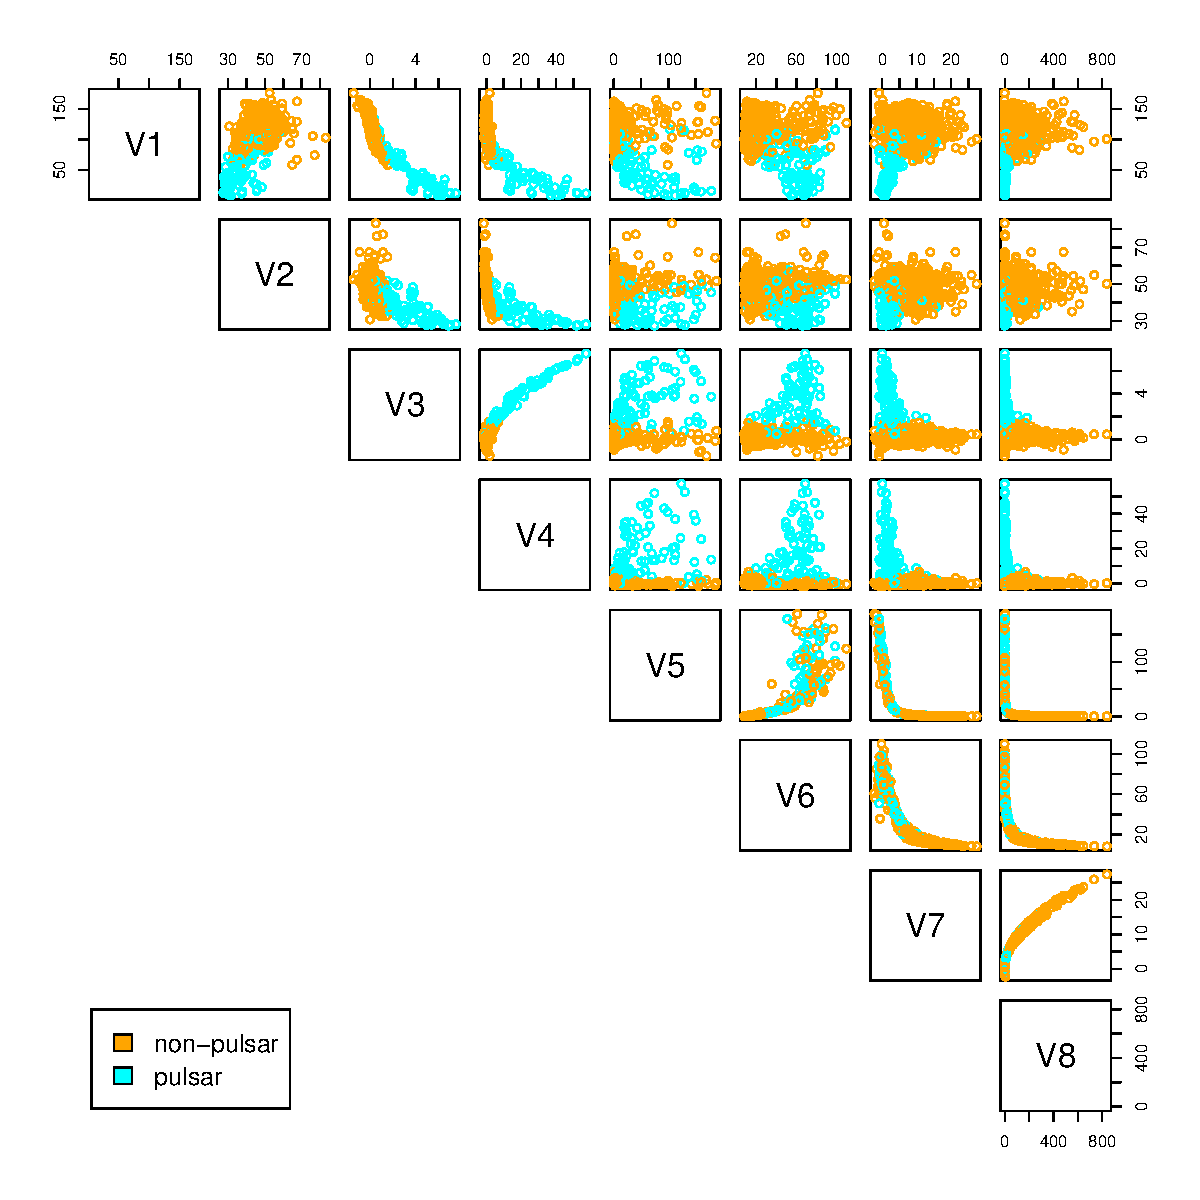
\includegraphics[width = 12cm]{scattermatrix}
\caption{Exploratory Data Analysis}
\label{fig:scatter}
\end{figure}
}
\begin{figure}[h!]
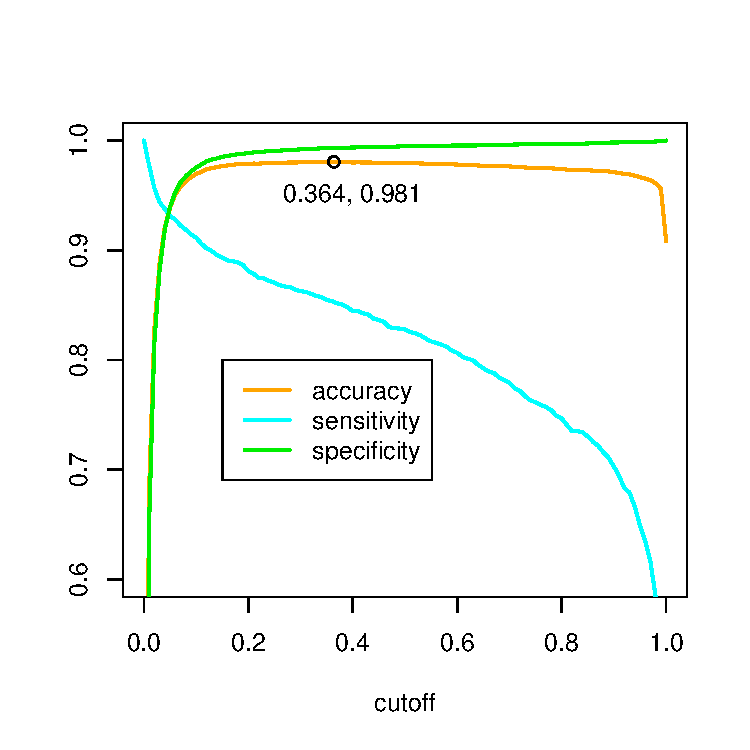
\includegraphics[width = 8.5cm]{cutoffs}
\caption{Performance of Model 1 for cutoffs $p_c \in [0,1]$}
\label{fig:cutoffs}
\end{figure}

\begin{figure}[h!]
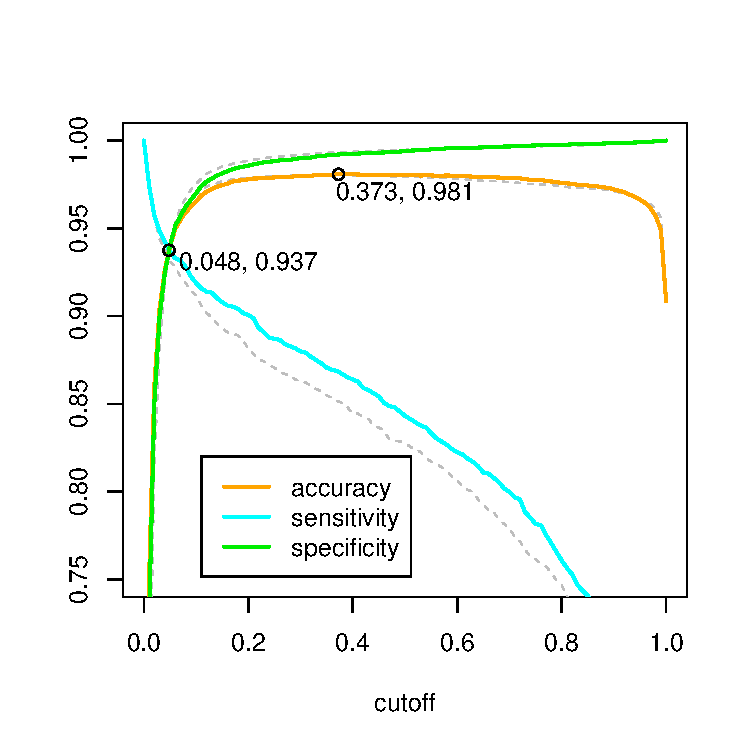
\includegraphics[width = 8.5cm]{cutoffs4}
\caption{Performance of Model 4 for cutoffs $p_c \in [0,1]$}
\label{fig:cutoffs4}
\end{figure}

~\\
\pagebreak
~\\
\pagebreak
\flushleft
\section*{Appendix: R Code}

The following code conducts data analysis and model formulation and diagnostics. 
\footnotesize
\begin{lstlisting}

    require(MASS)
    require(car)
    data <- read.csv("data/HTRU_2.csv", header=FALSE) #Change path for your system
    
    #### Functions ###########################################################
    logistic <- function(x) exp(x) / (1 + exp(x))
    
    logit <- function(p) log(p / (1 - p))
    
    get_confusion_matrix <- function(Y, Ypred){
      confusion <- rbind ( c(sum(!Ypred & !Y), sum(!Ypred & Y), sum(!Ypred)  ), 
                           c(sum(Ypred & !Y),  sum(Ypred & Y),  sum(Ypred)   ),
                           c(sum(!Y),          sum(Y),          length(Ypred)) )
      confusion <- confusion / length(Ypred)
      rownames(confusion) <- c("Predicted False", "Predicted True", "")
      colnames(confusion) <- c("Actually False", "Actually True", "")
      return(confusion)
    }
    
    get_accuracy <- function(Y, Ypred){
      return( sum(Ypred == Y) / length(Ypred))
    }
    
    print_model_details <- function(Y, Ypred){
      confusion <- get_confusion_matrix(Y, Ypred)
      print(round(confusion, 3))
      print(paste("Accuracy:", round(get_accuracy(Y, Ypred), 3)))
      print(paste("Specificity:", round(confusion[1, 1] / confusion[3, 1], 3)))
      print(paste("Sensitivity:", round(confusion[2, 2] / confusion[3, 2], 3)))
    }
    #### Exploratory Data Analysis ##########################################
    
    summary(data)
    summary(data[data$V9==T,])
    summary(data[data$V9==F,])
    set.seed(4607)
    indices <- sample(1:nrow(data), 1000, replace = F)
    # See also plotting code 
    
    # Note the collinearity issue: high correlation between (V3, V4) and (V7, V8). 
    round(cor(data), 2)
    
    Y <- data[, 9]
    
    #### Fit simple GLMs ####################################################
    # Fit a GLM with all 8 features and no interactions
    mdl <- glm(Y~., family = binomial, data = data[, 1:8])
    summary(mdl)
    
    # Accuracy and Confusion Matrix for this model as a classifier 
    #   with cutoff p = 0.5
    print_model_details(Y, mdl$fitted.values > 0.5)
    #   with cutoff p = 0.4 
    print_model_details(Y, mdl$fitted.values > 0.4)
    #   best cutoff
    accuracy <- Vectorize(function(cutoff){
      get_accuracy(Y, mdl$fitted.values > cutoff)
    })
    cutoff <- unlist(optimize(accuracy, c(0.1, 0.8), maximum = T)["maximum"])
    print_model_details(Y, mdl$fitted.values > cutoff)
    
    # Fit smaller GLMs by removing some of V3, V7, V8 
    #   Removing V8 gives a model with AIC 2634.3
    mdl1_v8 <- glm(Y~., family = binomial, data = data[,1:7])
    summary(mdl1_v8)
    #   Removing V7 gives a model with AIC 2632.1
    mdl2 <- glm(Y~.-V7, family = binomial, data = data[,1:8])
    summary(mdl2)
    #   Removing V3 and V7 should give a better model...
    #     but it leads to numerical issues. 
    badmdl1 <- glm(Y~.-V3-V7, family = binomial, data = data[,1:8])
    summary(badmdl1)
    #   Even removing only V3 has this issue. 
    badmdl2 <- glm(Y~.-V3, family = binomial, data = data[,1:8])
    summary(badmdl2)
    #     Diagnostics... 
    print_model_details(Y, badmdl2$fitted.values > 0.5)
    badmdl2$fitted.values[which(duplicated(badmdl2$fitted.values))]
    sum(badmdl2$fitted.values[which(duplicated(badmdl2$fitted.values))])
    badmdl2$linear.predictors[which(duplicated(badmdl2$fitted.values))]
    min(badmdl2$fitted.values[as.logical(Y)])
    max(badmdl2$fitted.values[as.logical(1-Y)])
    #   I believe that the issues arise because 11 observations are fitted to a
    #     value which is numerically equal to 1. I am not sure how to fix this
    #     problem.
    mdl3 <- glm(Y~.-V7-V4, family = binomial, data = data[,1:8])
    summary(mdl3)
    
    #   Stepwise selection finds the same model as mdl3
    if(F) stepAIC(mdl, direction = "both",  trace = F)
    
    #### Fit larger GLMs by adding interaction terms ####################
    # Fit a model with every interaction term. AIC 2466.8
    mdl4 <- glm(Y~.*., family = binomial, data = data[,1:8])
    summary(mdl4)
    
    # Stepwise model selection with interactions. Takes a while to run.
    if(F){ #Change to T to run this. 
      mdl5 <- stepAIC(mdl3, direction = "both",  trace = F)
      summary(mdl5)
    }
\end{lstlisting}
\normalsize
The following listing contains code for making the plots. 
\footnotesize
\begin{lstlisting}

#### Plotting ####

# Scatterplot matrix of V1-V8 with different colors for pulsars 
store <- par()$xpd # Store your xpd so it can be restored later
pdf(file = "figures/scattermatrix.pdf", width = 8, height = 8)
par(xpd = NA)
pairs(data[indices, 1:8], col = c("orange1", "cyan")[data[indices, 9] + 1],
      lower.panel = NULL#, panel = panel.smooth
)
legend( "bottomleft", fill = c("orange1", "cyan"), 
        legend = c("non-pulsar", "pulsar") )
dev.off()
par(xpd = store) # Restore your xpd
rm(store)

#   plotting all cutoffs in the interval [0, 1]
accuracy <- Vectorize(function(cutoff){
  get_accuracy(Y, mdl$fitted.values > cutoff)
})
sensitivity <- Vectorize(function(cutoff){ # true positives / actual positives
  confusion <- get_confusion_matrix(Y, mdl$fitted.values > cutoff)
  confusion[2, 2] / confusion[3, 2]
})
specificity <- Vectorize(function(cutoff){ # true negatives / actual negatives 
  confusion <- get_confusion_matrix(Y, mdl$fitted.values > cutoff)
  confusion[1, 1] / confusion[3, 1]
})

Y <- data[, 9]
mdl <- glm(Y~., family = binomial, data = data[, 1:8])

pdf(file = "figures/cutoffs.pdf", width = 5, height = 5)
plot(accuracy, 0, 1, lwd = 2, col = "orange1", xlab = "cutoff", ylab = "", 
     ylim = c(0.6, 1))
plot(sensitivity, 0, 1, add = T, lwd = 2, col = "cyan")
plot(specificity, 0, 1, add = T, lwd = 2, col = "green2")
legend(0.15, 0.8, legend=c("accuracy", "sensitivity", "specificity"),
       col=c("orange1", "cyan", "green2"), lwd = 2)
cutoff <- unlist(optimize(accuracy, c(0.1, 0.8), maximum = T)["maximum"])
points(cutoff, accuracy(cutoff))
text(0.4, 0.95, paste(round(cutoff, 3), ", ", round(accuracy(cutoff), 3), 
                      sep = ""))
dev.off()

\end{lstlisting}

\end{document}
